\documentclass[a4paper]{article}
\usepackage[francais]{babel}
\usepackage{fontspec}
\usepackage{enumitem}
\usepackage{authblk}
\usepackage{minted}
\usepackage{amsmath}
\usepackage{tabularx}
\newcolumntype{C}[1]{>{\centering\arraybackslash}p{#1}}
\graphicspath{{images/}}
\setlength{\parindent}{0pt}
\usepackage[left=2.5cm,top=2.5cm,right=2.5cm,bottom=2.5cm]{geometry}
 
\title{Projet VHDL}
\author{Mehmed Blazevic \& Orphée Antoniadis}
\date{Hepia 2018}
\begin{document}

\maketitle

\section{Introduction}
Dans le cadre du cours de VHDL, FPGA \& SoPC, il nous a été demandé de réaliser un projet. 
Le projet s'étale sur tout le semestre et le thème est libre. Nous avions tout de 
même certaines contraites:

\begin{itemize}
  \item Utiliser un périphérique existant (SPI, I2C, UART, ...)
  \item Créer un périphérique spécifique
\end{itemize}

\section{Notre idée}
Nous voulions travailler avec le musique. On pensait faire un instrument un peu 
différent de ce que l'on a l'habitude de voir. L'idée est de travailler avec l'espace. 
Nous avons décidé d'utiliser des capteurs ultrasons, afin de connaître la distance 
entre une main et ce capteur. En fonction de la distance que l'on mesure avec la main, 
nous avions dans l'idée de produire une notes de musique plus ou moins forte. 
L'idée était de placer 8 capteurs de distances allignés, afin de jouer avec un piano 
"virtuel". 

\subsection{Schema}

\begin{center}
\noindent\makebox[\textwidth]{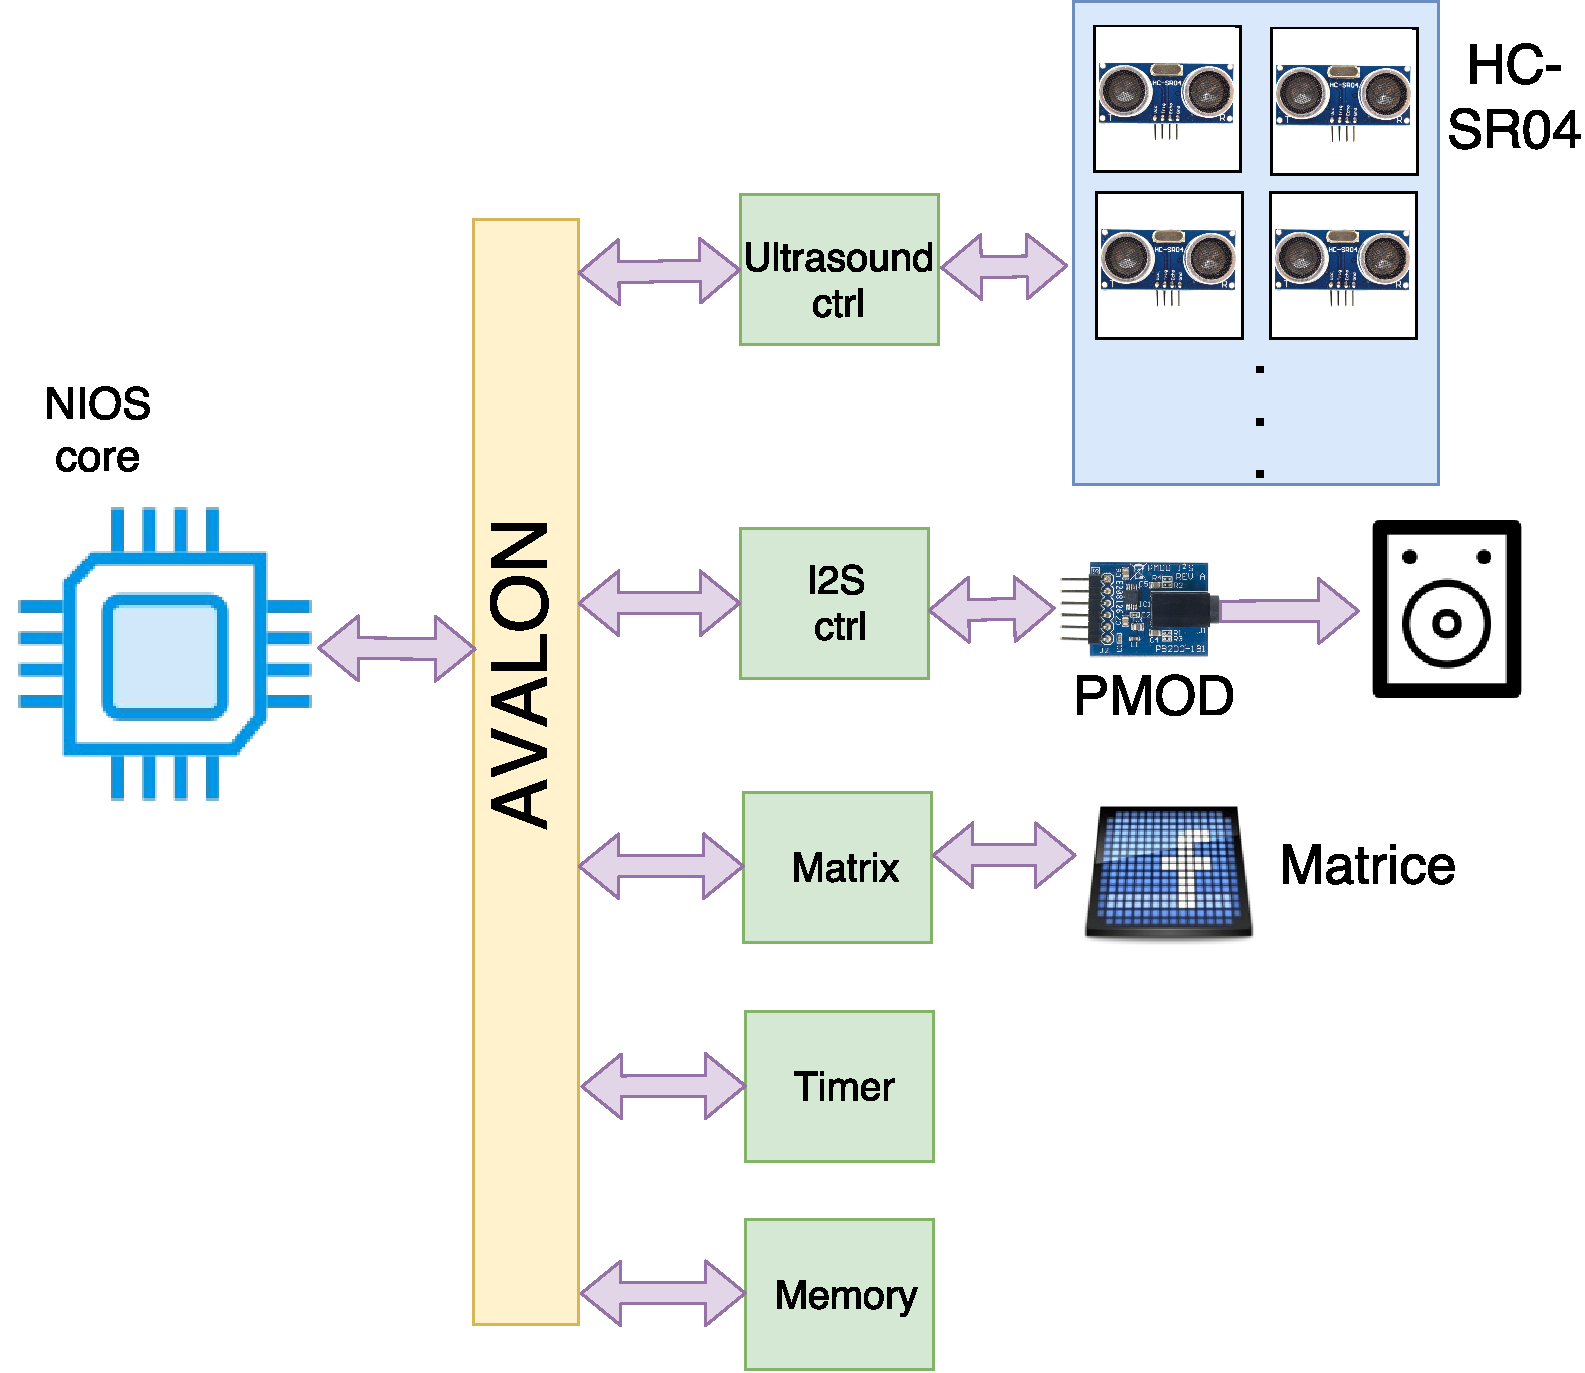
\includegraphics[width=350pt]{VHDL.pdf}}
\end{center}

\section{Drivers}
\subsection{Capteur ultrasons}
Le module ultrason que nous avons utilisé est le HCSR04 de Cytron Technologies.
Ce module est composé de 4 pins, le Vcc, le Gnd, une entrée appelée trig et une
sortie appelée echo. Il utilise son propre protocole qui très simple. Lorsque l'on
souhaite obtenir la distance, il faut mettre la pin trig à l'état haut pendant
10$\mu$s. Il faut ensuite remettre le trig à l'état bas, le module envoie une onde
ultrason et met la pin echo à l'état haut. L'echo est remis à l'état bas lorsque
l'onde ultrason a fait l'allé-retour. Pour obtenir la distance, il faut donc mesurer
le temps que l'echo a été à l'état haut. A noter que le module ultrason fonctionne
en 5V et la DE0 fonctionne en 3V3. Nous avons donc du faire un petit diviseur de tension
sur la pin echo. Le trig étant une entrée, les 3V3 de la FPGA suffisent à considérer
le signal comme étant à l'état haut. \\

Le driver que nous avons développé reproduit le comportement décrit ci-dessus.
Nous avons utilisé une machine à états pour le reproduire. Pour éliminer le bruit,
nous faison une moyenne sur 100 échantillons. L'interface avalon dévéloppée est
très simple elle aussi. Il n'y a qu'un seul registre en lecture seule. Ce registre
contient le nombre de coups d'horloges de la DE0 pendant lesquels l'echo était à
l'état haut. Au niveau du code C il suffit de convertir ces coups d'horloge et
utiliser la vitesse du son afin d'obtenir la distance entre le module et l'obstacle.
Notre driver fonctionnait mais nous avons remarqué que la distance calculée n'était
pas très précise mais assez pour notre projet.

\subsection{I2S}


\end{document}
